\subsection{Subsection}

Figure reference: \ref{fig:name}.

\begin{wrapfigure}{R}{0.5\textwidth}
\centering
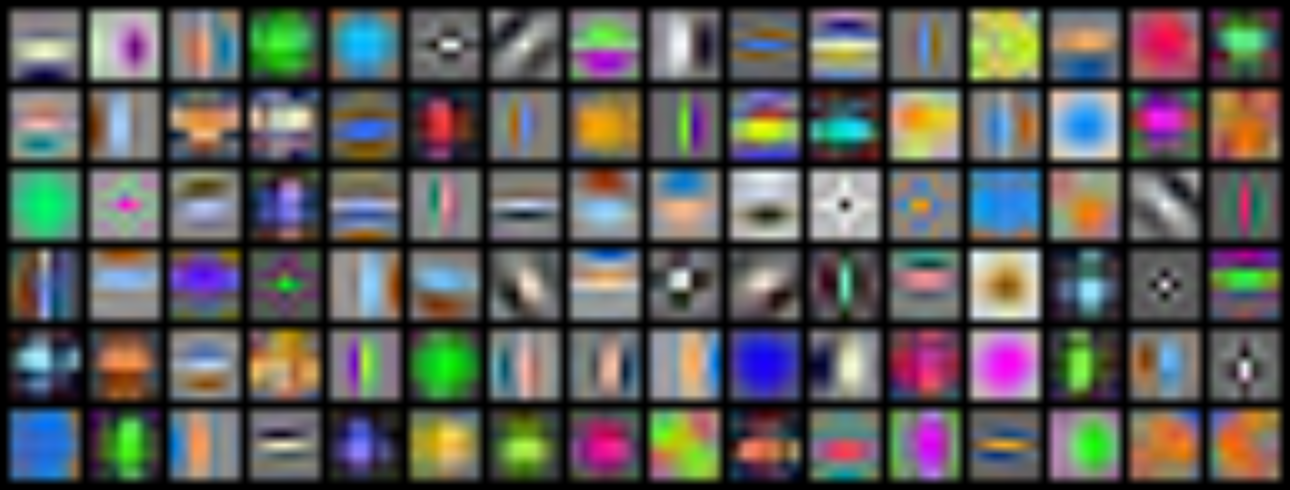
\includegraphics[width=0.48\textwidth]{./figures/cifar10_layer1_filters_7x7_11m-09d-21h-38m-00s.png}
\caption{Caption.}
\label{fig:name}
\vspace{-0.5cm}
\end{wrapfigure}

Table reference: \ref{tab:name}

\begin{table}[b]
\begin{center}
    \caption{Table.}
    \label{tab:name}
    \begin{tabular}{ |l | c | c | c | c |}
    \hline
    \multicolumn{1}{|p{5cm}|}{\raggedright Unsupervised to supervised ratio \\ (Samples per Class)}
& \multicolumn{1}{|p{1cm}|}{\centering 50:1 \\ (100)}
& \multicolumn{1}{|p{1cm}|}{\centering 10:1 \\ (500)}
& \multicolumn{1}{|p{1cm}|}{\centering 5:1  \\ (1000)}
& \multicolumn{1}{|p{1cm}|}{\centering 1:1  \\ (5000)} \\ \hline
     Tanh CNN & 44.48 \% & --- & 64.77 \% & 77.50 \% \\ %\hline
     Tanh CAE & 47.70 \% & --- & 65.65 \% & 78.20 \% \\ \hline
     Zero-bias CNN  & 47.01 \% & 64.76 \%& 73.30 \% & 82.73 \% \\
     \bf Zero-bias CAE  & \bf 55.45 \% & \bf 68.42 \% & \bf 74.06 \% & \bf 83.64 \% \\ \hline
    \end{tabular}
\end{center}
\end{table}